\documentclass{assignment}
\usepackage{amsmath}
\usepackage{lipsum}
\usepackage{multicol}
\usepackage{fancyhdr}
\usepackage{graphicx}
\usepackage{blindtext}
\usepackage[dvipsnames]{xcolor}
\usepackage{enumitem}

\fancyhf{}% Clear all headers/footers
\fancyhead[L]{Tillämpad Datalogi \\ DD1320}\fancyhead[R]{\textbf{Lucas Frykman} \\ lfrykman@kth.se}
\fancyfoot[C]{\thepage}
\setlength{\headheight}{26pt}
\pagestyle{fancy}
\thispagestyle{plain}

\begin{document}
\assignmentTitle
{Lucas Frykman}{0210127650}
{SF1550}
{Olof Runborg}
{assets/KTH_logga.png}
{Numeriska metoder, grundkurs}
{Laboration 1}

\section*{Uppgift 1}

\begin{itemize}
    \item Hur många nollställen: 6
    \begin{figure}[!h]
        \caption{Rötter till grafen $f(x)=x^2-8x-5sin(3x+1)+12$}
        \centering
        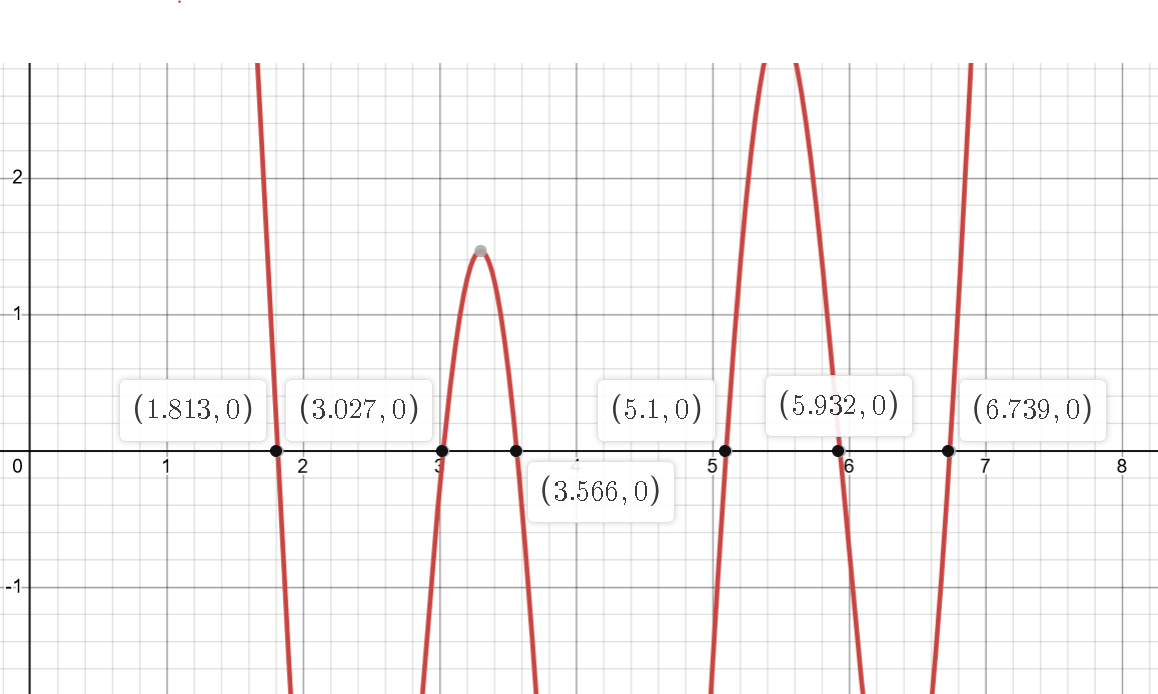
\includegraphics[width=120mm,height=100mm]{assets/rootsgraph.PNG}
    \end{figure}
    \\ Som ni ser i Figure 1 det finns 6 rötter till funktionen nämligen 
    $x_0 \approx [1.81,3.027,3.56,5.10,5.93,6.73]$
    \newpage
    \item Motivera varför fixpunkt: 
    \begin{align}
        f(x^{*})=0 \Leftrightarrow
        \\ x^2-8x-5sin(3x+1)+12 = 0 \Leftrightarrow \nonumber
        \\ x^2+4x-5sin(3x+1)+12 = 12x \Leftrightarrow \nonumber
        \\ \underbrace{\frac{1}{12}x^2+\frac{1}{3}x-\frac{5}{12}\sin(3x+1)+1}_{\phi (x)} = x
    \end{align}

    \item Vilka nollställen kan det hitta: 
    \\ Vi vet att 

    \begin{align}
        \phi ' (x)=\frac{d}{dx} (\frac{1}{12}x^2+\frac{1}{3}x-\frac{5}{12}\sin(3x+1)+1)
        =\frac{1}{6}x+\frac{1}{3}-\frac{5}{4}\cos(3x+1)
    \end{align}
    \\som erhåller att metoden konvergerar till 3 olika punkter och divergerar till resten
    \begin{align*}
        |\phi ' (1.81)| & \approx 0.601 < 1 &\textbf{konvergerar}
        \\ |\phi ' (3.027)| & \approx 1.8 > 1 &\textbf{divergerar}
        \\ |\phi ' (3.56)| & \approx 0.13 < 1 &\textbf{konvergerar}
        \\ |\phi ' (5.10)| & \approx 2.2 > 1 &\textbf{divergerar}
        \\ |\phi ' (5.93)| & \approx 0.073 < 1& \textbf{konvergerar}
        \\ |\phi ' (6.73)| & \approx 2.3 > 1 &\textbf{divergerar}
    \end{align*}

    \item Hur ska fel termen avta?
    \\fixpunkt iterationen ska ha linjär konvergensordning eftersom 
    $\phi ' (x^{*})\neq 0$
    % \item Stämmer tumregeln för Newtons metod att antalet korrekta siffror dubblas i varje iter
    % \item Vilken av metoderna konvergerar snabbast?
    \newpage
    \item Uppskatta metodernas konvergensordning med hjälp av figuren. Stämmer det med
    teorin
    \\
    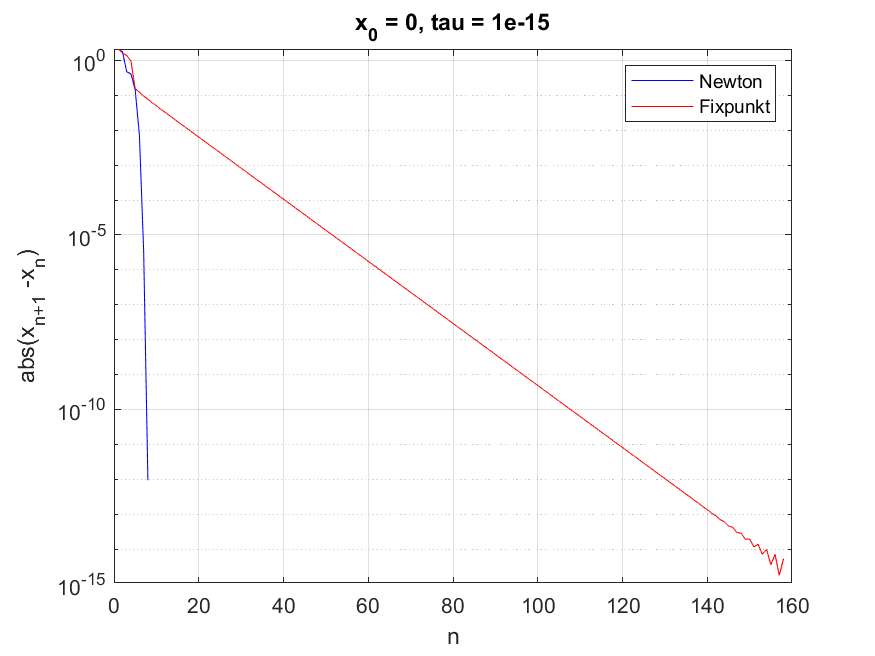
\includegraphics[]{assets/konvplot1.png}
    Ja det syns tydligt i grafen att fixpunkt iterationen bildar en linje
    och newtonsmetod bildar en parabola. 
    Det här stämmer med teorin eftersom newton har konvergens ordningen
    2 och fixpunkt iterationen är 1.
\end{itemize}

\newpage
\section*{Uppgift 2}
\begin{itemize}
    \item Hur många lösningr finns det? Det finns 3 lösningar.
\end{itemize}

\section*{Uppgift 3}

\begin{itemize}
    \item Plotta både tornen
    \\
    \begin{figure}[!h]
        \caption{eiffel2.mat med ändring vid nod j=261}
        \centering
        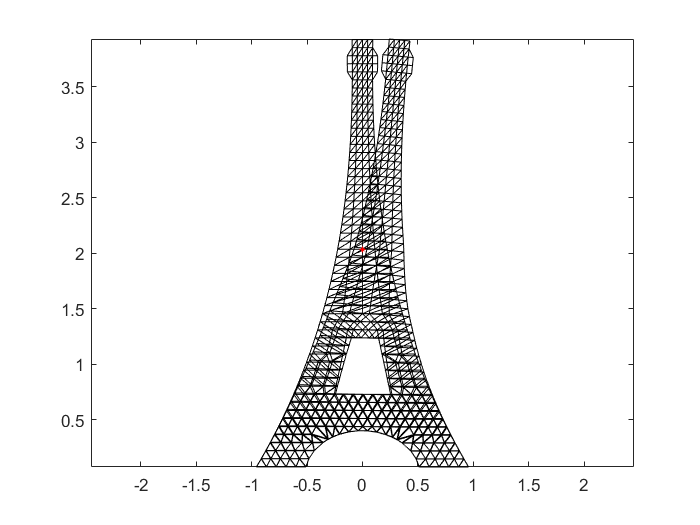
\includegraphics{assets/tornen.png}
    \end{figure}
    % \item Varför går det snabbare att lösa problemet med LU-faktorisering?
    % \item Vilken metod löser problemet snabbast? (Med/utan LU? Full/gles lösar) tidskomplexitet
    % \item För vilken modell blir tidsvinsten störst? Varför?    
\end{itemize}
Det går snabbare eftersom att lösa 
\[ M\mathsf{x}=b \] har komplexitet $\mathcal{O}(n^3)$
men om matrisen är triangulär så är det $\mathcal{O}(n^2)$
Vilket kan implementeras med $M=LU$ faktorisering
genom 
\[LU\mathsf{x}=b\]
som kan implementeras med koden 

\lstinputlisting[language=Matlab,caption=LU implementation]{assets/Q1D1.m}
där lösningen till $b$ har komplexitet $\mathcal{O}(2n^2)$
men komplixtet till koden ovan är faktiskt $\mathcal{O}(n^3+2n^2)$ som är faktiskt långsammare.
Tidsvinsten visar sig om man itererar för många olika $b$ säg j gånger.
Så blir det $\mathcal{O}(n^3+2jn^2) < \mathcal{O}(jn^3)$ när $j$ är tillräckligt stort.
\end{document}